
\chapter{Podstawy teoretyczne}
\subsection{Logika}
Aby mówić o werfikacji modeli musimy się wyposażyć w  elementarz teoretyczny. Potrzebne nam są podstawowe 
definicje i pojęcia zanim zaczniemy mówić o skomplikowanych modelach. Ważne jest również 
wprowadzenie i usystematyzowanie informacji z różnych źródeł. Rodział ten został oparty 
na świetnej książce ~\cite{Jamroga} i będzie stanowił fundament dalszej tej pracy.
Podstawowe elementy logiki można znaleźć w świetnej książce ~\cite[Podstawy Logiki]{batog1994podstawy} do której serdecznie
odsyłam.

 System wieloagentowy (ang. multi-agent system, MAS) to system składający się z autonomicznych podmiotów, działających 
 w tym samym środowisku. Jest on wykorzystywany do modelowania i opisywania systemów z którymi 
 spotykamy się w świecie informatyki i nie tylko. Agenci mogą podejmować akcje w jednym 
środowisku. Przykładem takiego środowiska mogą być wybory, gdzie grupa $n$ wyborców 
(agentów) bierze udział w procesie wyborczym.

Logika modalna którą będziemy się posługiwali jest rozszerzeniem klasycznej logiki 
o nowe operatory $\Box$ i konieczności $\diamond$. Formuła $\Box \phi$ oznacz, że $\phi$ 
jest prawdziwa zawsze w każdym stanie. Formuła $\diamond \phi$ oznacza, że $\phi$ jest prawdziwe 
w pewnym stanie. Spełniona jest przy tym zasada 
\begin{equation*}
    \lozenge \varphi \iff \neg \Box \neg \varphi
\end{equation*}

Wprowdzaimy teraz definicję modele Kripkiego.
\begin{definition}[Model Kripkiego]
    Niech \( PV = p, p', p'', \ldots \) będzie zbiorem zmiennych 
    zdaniowych. Modele logiki modalnej nazywane są modelami Kripkego lub modelami możliwych 
    światów i obejmują zbiór możliwych światów (lub stanów) \( St \),
     modalną relację dostępności \( R \subseteq St \times St \) oraz interpretację 
     zmiennych \( \mathcal{V} : PV \rightarrow 2^{St} \).
\end{definition}

Jeśli trójka $M=(St,R,V)$ będzie modelem kripkiego i $q$ będzie możliwym słowem w $M$,
to prawdziwość formuły $M,q$ jest dana relacją $ \models $ i jest zdefiniowana indukcyjnie 
przez zasady
\[
\begin{array}{ll}
M, q \models p & \text{wtedy i tylko wtedy, gdy} \quad q \in V(p), \quad \text{dla} \quad p \in \mathcal{PV}; \\
M, q \models \neg \varphi & \text{wtedy i tylko wtedy, gdy} \quad \text{nie} \quad M, q \models \varphi \quad (\text{często pisane} \quad M, q \not\models \varphi); \\
M, q \models \varphi \land \psi & \text{wtedy i tylko wtedy, gdy} \quad M, q \models \varphi \quad \text{i} \quad M, q \models \psi; \\
M, q \models \varphi \lor \psi & \text{wtedy i tylko wtedy, gdy} \quad M, q \models \varphi \quad \text{lub} \quad M, q \models \psi; \\
M, q \models \Box \varphi & \text{wtedy i tylko wtedy, gdy} \quad \text{dla każdego} \quad q' \in St \quad \text{takiego, że} \quad q R q', \quad \text{mamy} \quad M, q' \models \varphi; \\
M, q \models \Diamond \varphi & \text{wtedy i tylko wtedy, gdy} \quad \text{dla pewnego} \quad q' \in St \quad \text{takiego, że} \quad q R q', \quad \text{mamy} \quad M, q' \models \varphi.
\end{array}
\]

Prosty przykład modelu Kripkiego może wyglądać tak:

\begin{figure}[H]
    \centering
    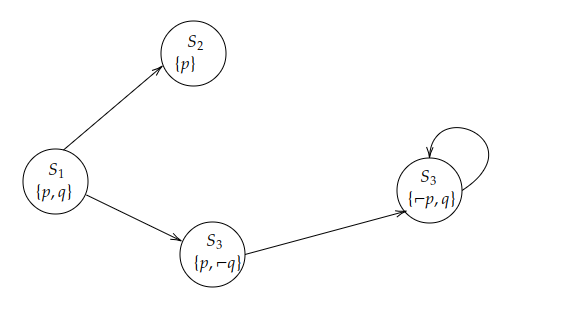
\includegraphics[width=\linewidth]{figures/kripke_model.png}
    \caption{Model Kripkiego}
    \label{fig:enter-label}
  \end{figure}

  W tym przypadku zbiorem stanów jest zbiór $St=\{S_{1}, S_{2}, S_{3}, S_{4}\}$.
  Relacja dostępności wygląda tak: $R=\{(S_{1}, S_{2}), (S_{1}, S_{3}), (S_{3}, S_{4})\}$.
  Zbiór $PV$ możemy odczytać bezpośrednio z diagramu. Formuła 
  \begin{equation*}
    \Box (p \lor q)
  \end{equation*}
  jest prawdziwa. Wynika to z tego, że wyrażenie $p \lor q$ jest prawdziwe w każdym stanie na diagramie.
  Formuła ta jest równoważna forumle 
  \begin{equation*}
    \neg \Diamond \neg(p \lor q)
  \end{equation*}
  poprzez zastosowanie podwójnej negacji.
\subsection{Uczenie ze wzmocnieniem}. 

Uczenie ze wzmocnieniem to dynamicznie rozwijająca się część sztucznej inteligencji.
Jest to proces, w którym agent ucz się jakie działania podejmować w środowisku, 
aby uzyskać jak największą nagrodę. Agent uczy się w pewien sposób metodą prób i błędów,
nie jest dla niego jasne które akcje przyniosą mu największe nagrody. Problemy ten 
charakterysuje się opóźnioną nagrodą. Oznacza to, że za akcję podjęte w pewnym momencie 
wpływają nie tylko na bieżącę nagrody, ale również na przyszłe stany i nagrody z nimi związane.

Uczenie ze wzmocnieniem samo w sobie jest szerokim zagadnieniem, zawiera w sobie zarówno sam problem,
klasę metod którą są w stanie rozwiązać problem jak i całą dziedzinę nauki. Kluczowym aspektem 
jest rozróżnienie pomiędzy problemem a metodami służącymi do jego rozwiązania.

Problemy uczenia ze wzmocnieniem formalizujemy za pomocą procesów decyzyjnych Markova.
Agent musi w pewien sposób odczuwać stan środowiska, podejmować działania wpływające na środowisko 
i mieć cele związane ze stanem środowiska. Procesy decyzyjne Markova uwzględniają te trzy aspekty.

Uczenie ze wzmocnieniem rózni się od dobrze znanego uczenia nadzorowanego, w którym system uczy 
się bazując na podstawie poetykietownych przez nadzorcę przykładów ze zbioru uczącego.
Różni się również od uczenia nienadzorowanego, które zazwyczaj polega na znajdowaniu 
struktur i wzorców w nieoznaczonych zbiorach danych. Uczenie ze wzmocnieniem dąży 
uzyskania jak największej nagrody, a nie do odrykwania struktur w zbiorach danych.

Jednym z wyzwań przed którym stajemy wykorzystując uczenie ze wzmocnieniem jest przetarg 
pomiędzy eksploracją i eksplatacją. Agent musi wybierać pomiędzy akcjami, które przyniosły mu już 
nagrodę, a wybieraniem nowych akcjii i stanów których jeszcze nie zna, a te mogą mu przynieść 
nagrody w przyszłości. Ani eksplatacją ani eksploracja nie mogą być wykonywane wyłącznie,
gdyż uniemożliwi to agentowi uzsykanie celu.

\subsection{Algorytmy uczenie ze wzmocnieniem}
Podczas badań zostały wykorzystane różne algorytmy uczenia ze wzmocnieniem. Poniżej zostanie dokonana
ich krótka charakterystyka.

\subsection*{AlphaZero}
Algorytm AlphaZero jest zaawansowany algorytmem uczenia ze wzmocnieniem. Zmień on sposób myślenia 
w tej gałęzi nauki. Pokazał on, że sztuczna inteligencja jest w stanie osiągnąć poziom nie możliwy do 
osiągnięcia dla człowieka w grach planszowych dla dwóch graczy. W artykule ~\cite{alpha_zero} zaprezentowane
zostałe osiągnięcia dla dobrze znanych gier jak szachy, shogi czy go. Algorytm ten nauczył się grać bez 
wiedzy dziedzinowej. Proces nauki polega na grze z samym sobą, co stopniowo prowadzi do polepszania 
swoich umiejętności. AlphaZero składa się z kilku kluczowych elementów.

Głęboka sieć nueronowa ocenia pozycję na planszy, prognozuje prawodopodobieństwa wykonania ruchu i ocenia wynik gry.
Sieć możemy oznaczyć jako $(p,v)=f_{\theta}(s)$. Parametry $\theta$ to parametry sieci, $s$ to stan gry przyjmowany na wejście,
a wynikiem działania sieci jest wektor prawdopodobieństwa $p$ oznaczający prawdopodobieństwo wykonania ruchów oraz 
wartość oczekiwaną pozycji $v$.

Klasyczny algorytm przeszukiwania drzewa \textit{alfa-beta} został zastąpiony przez \textit{Monte Carlo Tree Search (MCTS)}
który jest bardziej ogólnym podejściem. Każda symulacja w MCTS wybiera ruchy na podstawie małej liczby odwiedzin (ruchów dotychczas mało eksplorowanych),
 wysokiego prawdopodobieństwa ruchu i wysokiej wartości stanu.

 Parametry $\theta$ sieci neuronowej są aktualizowane na podstawie wyników rozegranych gier oraz różnicy pomiędzy 
 przewidywanym wynikiem $v$ a rzeczywistym wynikiem gry. Minimalizowana jest minimalizacja funkcji straty, która składa 
 się z błędu średniokwadratowego i straty entropii krzyżowej 
 \begin{equation*}
    l = (z-v)^{2} - \sum_{a} p_{a} \log{q_{a} + c ||\theta||^{2}}
 \end{equation*}
 gdzie $c$ jest parametrem regularyzacji $L2$.

 Alphazero rozpoczyna proces treningu od losowych ruchów bez posiadania wiedzy domenowej oprócz reguł gry. Wraz z procesem 
 treningu AlphaZero zwiększa swoje umięjętności wskutek aktualizacji wag modelu. Algorytm ten jest algorytmem który bardzo szybko 
 się uczy. Dowodzi tego fakt, że zaledwie po czterech godzinach treningu model był w stanie pokonać dotychczas najlepszy 
 silnik szachowy \textit{Stockfish}